\documentclass{article}

\usepackage{graphicx}
\usepackage{tikz}
\usepackage{tikzsymbols}
\usetikzlibrary{calc,patterns,shapes.geometric}
\pagestyle{empty}
\usepackage[margin=0pt]{geometry}
\geometry{papersize={14in,12in}}

\def\centerarc[#1](#2)(#3:#4:#5){\draw[#1] ($(#2)+({#5*cos(#3)},{#5*sin(#3)})$) arc (#3:#4:#5);}

\begin{document}
	\begin{figure}
		\centering
		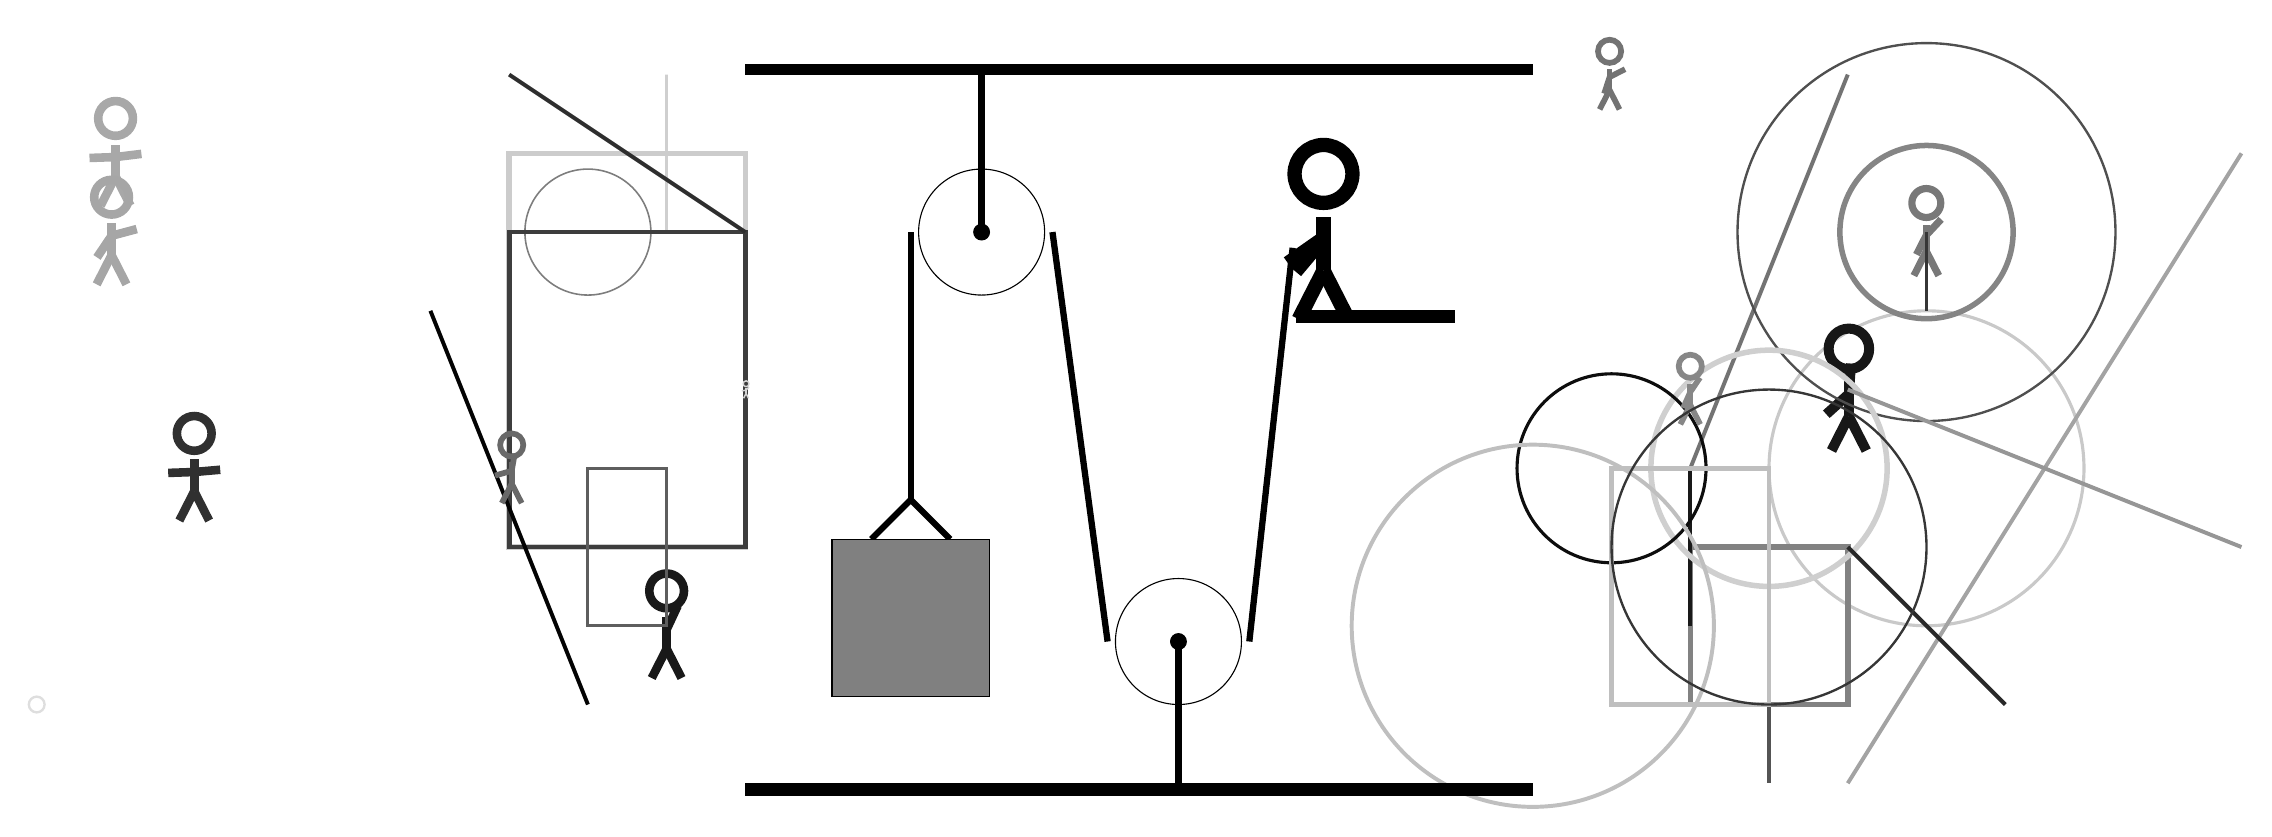
\begin{tikzpicture}
			%%%%% START %%%%%
			
			\draw[fill=black] (-2, 9) rectangle (8, 9.125);
			
			\draw (3.5, 1.8) circle (0.8);
			\draw[fill=black] (3.5, 1.8) circle (0.1);
			\draw[line width=0.8mm] (3.5, 1.8) -- (3.5, 0);
			
			\draw (1, 7) circle (0.8);
			\draw[fill=black] (1, 7) circle (0.1);
			\draw[line width=0.8mm] (1, 9) -- (1, 7);
			
			\draw[line width=0.8mm](-0.4, 3.1) --  (0.1, 3.6) -- (0.6, 3.1);
			\draw[fill=black!50] (-0.9, 3.1) rectangle (1.1, 1.1);
			
			\draw[line width=0.8mm](0.1, 7) -- (0.1, 3.6);
			\centerarc[line width=0.8mm](1, 7)(180:0:0.9)
			\draw[line width=0.8mm](1.9, 7) -- (2.6, 1.8);
			\centerarc[line width=0.8mm](3.5, 1.8)(180:360:0.9)
			\draw[line width=0.8mm](4.4, 1.8) -- (4.95, 6.8);
			
			\draw [line width=0.4mm, color=black!21](13, 4) circle (2.0);
			
			\node[line width=0.5mm, color=black!53] at (13, 7) {\Strichmaxerl[5][63][47]};
			\node[line width=0.4mm, color=black!91] at (12, 5) {\Strichmaxerl[7][42][86]};
			\draw[line width=0.5mm, color=black!55](12, 9) -- (10, 4);
			\node[line width=0.4mm, color=black!90] at (-3, 2) {\Strichmaxerl[6][90][65]};
			
			\draw[line width=0.5mm, color=black!36](12, 0) -- (17, 8);
			\node[line width=0.2mm, color=black!34] at (-10, 8) {\Strichmaxerl[6][2][7]};
			\node[line width=0.6mm, color=black!81] at (-9, 4) {\Strichmaxerl[6][2][5]};
			\node[line width=0.5mm, color=black!35] at (-10, 7) {\Strichmaxerl[6][56][15]};
			\draw[line width=0.7mm, color=black!49] (10, 3) rectangle (12, 1);
			\draw [line width=0.7mm, color=black!48](13, 7) circle (1.1);
			\draw[line width=0.3mm, color=black!19] (-3, 7) rectangle (-3, 9);
			\draw [line width=0.3mm, color=black!69](13, 7) circle (2.4);
			
			\draw[line width=0.5mm, color=black!90](10, 4) -- (10, 2);
			\draw [line width=0.7mm, color=black!19](11, 4) circle (1.5);
			\draw[line width=0.3mm, color=black!53] (-4, 8) rectangle (-3, 8);
			
			\draw [line width=0.2mm, color=black!51](-4, 7) circle (0.8);
			\draw[line width=0.5mm, color=black!79](13, 6) -- (13, 7);
			\draw[line width=0.7mm, color=black!20] (-2, 3) rectangle (-5, 8);
			\draw [line width=0.4mm, color=black!95](9, 4) circle (1.2);
			\draw[line width=0.6mm, color=black!76] (-2, 3) rectangle (-5, 7);
			
			\node[line width=0.5mm, color=black!16] at (-2, 5) {\Strichmaxerl[1][10][48]};
			
			\draw [line width=0.5mm, color=black!25](8, 2) circle (2.3);
			\draw[line width=0.5mm, color=black!41](12, 5) -- (17, 3);
			\draw[line width=0.4mm, color=black!63] (-4, 4) rectangle (-3, 2);
			\draw[line width=0.5mm, color=black!67](11, 3) -- (11, 0);
			\node[line width=0.2mm, color=black!55] at (9, 9) {\Strichmaxerl[4][72][27]};
			\draw[line width=0.5mm, color=black!82](-2, 7) -- (-5, 9);
			\draw[line width=0.5mm, color=black!84](12, 3) -- (14, 1);
			
			\node[line width=0.7mm, color=black!47] at (10, 5) {\Strichmaxerl[4][66][56]};
			\draw[line width=0.6mm, color=black!25] (9, 4) rectangle (11, 1);
			
			\draw[line width=0.5mm, color=black!99](-6, 6) -- (-4, 1);
			\draw [line width=0.3mm, color=black!13](-11, 1) circle (0.1);
			\draw [line width=0.3mm, color=black!79](11, 3) circle (2.0);
			\node[line width=0.3mm, color=black!59] at (-5, 4) {\Strichmaxerl[4][16][80]};
			
			\node at (5.3, 7) {\Strichmaxerl[10][35][-130]};
			\draw[fill=black] (5, 6) rectangle (7, 5.85);
			
			\draw[fill=black] (-2, 0) rectangle (8, -0.15);
			
			%%%%% END %%%%%
		\end{tikzpicture}
	\end{figure}	
\end{document}